\documentclass{sigchi}

% Use this command to override the default ACM copyright statement (e.g. for preprints). 
% Consult the conference website for the camera-ready copyright statement.


%% EXAMPLE BEGIN -- HOW TO OVERRIDE THE DEFAULT COPYRIGHT STRIP -- (July 22, 2013 - Paul Baumann)
% \toappear{Permission to make digital or hard copies of all or part of this work for personal or classroom use is 	granted without fee provided that copies are not made or distributed for profit or commercial advantage and that copies bear this notice and the full citation on the first page. Copyrights for components of this work owned by others than ACM must be honored. Abstracting with credit is permitted. To copy otherwise, or republish, to post on servers or to redistribute to lists, requires prior specific permission and/or a fee. Request permissions from permissions@acm.org. \\
% {\emph{CHI'14}}, April 26--May 1, 2014, Toronto, Canada. \\
% Copyright \copyright~2014 ACM ISBN/14/04...\$15.00. \\
% DOI string from ACM form confirmation}
%% EXAMPLE END -- HOW TO OVERRIDE THE DEFAULT COPYRIGHT STRIP -- (July 22, 2013 - Paul Baumann)


% Arabic page numbers for submission. 
% Remove this line to eliminate page numbers for the camera ready copy
\pagenumbering{arabic}


% Load basic packages
\usepackage{balance}  % to better equalize the last page
\usepackage{graphics} % for EPS, load graphicx instead
\usepackage{times}    % comment if you want LaTeX's default font
\usepackage{url}      % llt: nicely formatted URLs

% llt: Define a global style for URLs, rather that the default one
\makeatletter
\def\url@leostyle{%
  \@ifundefined{selectfont}{\def\UrlFont{\sf}}{\def\UrlFont{\small\bf\ttfamily}}}
\makeatother
\urlstyle{leo}


% To make various LaTeX processors do the right thing with page size.
\def\pprw{8.5in}
\def\pprh{11in}
\special{papersize=\pprw,\pprh}
\setlength{\paperwidth}{\pprw}
\setlength{\paperheight}{\pprh}
\setlength{\pdfpagewidth}{\pprw}
\setlength{\pdfpageheight}{\pprh}

% Make sure hyperref comes last of your loaded packages, 
% to give it a fighting chance of not being over-written, 
% since its job is to redefine many LaTeX commands.
\usepackage[pdftex]{hyperref}
\hypersetup{
pdftitle={SIGCHI Conference Proceedings Format},
pdfauthor={LaTeX},
pdfkeywords={SIGCHI, proceedings, archival format},
bookmarksnumbered,
pdfstartview={FitH},
colorlinks,
citecolor=black,
filecolor=black,
linkcolor=black,
urlcolor=black,
breaklinks=true,
}

% create a shortcut to typeset table headings
\newcommand\tabhead[1]{\small\textbf{#1}}


% End of preamble. Here it comes the document.
\begin{document}

\title{MindMargin: Capturing Reader Engagement with an Article-Adjacent Commenting Platform}

\numberofauthors{3}
\author{
  \alignauthor 1st Author Name\\
    \affaddr{Affiliation}\\
    \affaddr{Address}\\
    \email{e-mail address}\\
    \affaddr{Optional phone number}
  \alignauthor 2nd Author Name\\
    \affaddr{Affiliation}\\
    \affaddr{Address}\\
    \email{e-mail address}\\
    \affaddr{Optional phone number}    
  \alignauthor 3rd Author Name\\
    \affaddr{Affiliation}\\
    \affaddr{Address}\\
    \email{e-mail address}\\
    \affaddr{Optional phone number}
}

\maketitle

\begin{abstract}

\end{abstract}

\keywords{
	Guides; instructions; author's kit; conference publications;
	keywords should be separated by a semi-colon.
	\textcolor{red}{Mandatory section to be included in your final version.}
}

\category{H.5.m.}{Information Interfaces and Presentation (e.g. HCI)}{Miscellaneous}

See: \url{http://www.acm.org/about/class/1998/}
for more information and the full list of ACM classifiers
and descriptors. 
\textcolor{red}{Mandatory section to be included in your
final version. On the submission page only the classifiers'
letter-number combination will need to be entered.}

\section{Introduction}

News pages, media sites, online shops, blogs and social networks support the ability to give content-related feedback in the form of comments. Commenting systems on these sites are traditionally featured under, and separate from, the main content. This structure parallels the relationship between content and comments, as interactions with comments are markedly secondary to the primary task of reading or browsing primary content. However, studies on Fluid Documents and annotation interfaces that challenge typographic conventions, such as discussion boards and footnotes, reveal limitations in the traditional vertical interface and suggest alternative horizontal layouts~\cite{FluidDocs,NewsInterfaces,NB,AnnotationsStudents,Brush,Guzdial,van}. 

The Fluid Documents project aims to make information added into a page easier to locate in its source document by adjusting the typography of page. One specific study found that a fluid margin interface, as opposed to a fluid interline or overlay interface, had minimal disturbance to the user, because it did not move or occlude the primary text with the secondary text~\cite{FluidDocs}. 

The concept of anchoring annotations to references in a text has been known to qualitatively improve conversation among readers because it makes understanding the context of a comment cognitively easier~\cite{Brush,Guzdial,van}. Another study compares the four leading annotation interfaces: footnotes, interlinear commentary, ``sticky-note`` annotations, and marginal comments, concluding that the marginal interface is superior in minimizing distraction and enhancing visibility. The marginal interfaces studied, however, interact with the primary text. They are tagged to boxes around the referenced content to indicate where they are anchored~\cite{AnnotationsStudents}. 

We have thus chosen to anchor comments in MindMargin with a faint dotted line to the edge of the article that corresponds to the y-coordinate of its reference, yet still avoids disturbing the primary text.

While online commenting provides an opportunity for readers to express their views and engage in lively discussion with others, the comments section of many websites has become a popular space for “flame wars.” The social act of “flaming,” or the posting of offensive content, regularly devolves into hostile fights among multiple users, diverting a legitimate discussion topic to an unrelated and often emotionally charged digression. This behavior is examined closely in many research fields, including user interface design, communications, and psychology~\cite{FlamingComp,FlamingPsych,FlamingSoftware,FlamingCommunications}. 

Evidence in educational research, however, has shown that anchored annotated notes foster a deeper understanding of the text and facilitate more thoughtful teacher-to-student and peer-to-peer discussions~\cite{AnnotationsStudents,NB}. Studies on balancing people’s skewed opinions also suggest exposing readers to a variety of relevant perspectives so that they consider views that exist beyond a single article and author’s scope~\cite{Politics,NewsCube,ConsiderIt}. 

Thus, while current commenting platforms often fail at drawing people into sensible and relevant conversation, we offer evidence to suggest a horizontal interface such as MindMargin can change people’s views and actions, and thus address this societal problem. From our evaluation and user study, it appears that people with prior exposure to the issue in the article become more moderate in their opinions, reporting less polar views than those using a traditional vertical interface.

\subsection{Hypotheses}
We propose two hypotheses for MindMargin's effect on its users in comparison to the traditional vertical interface:
\begin{enumerate}
\item Users of MindMargin will develop more thoughtful and nuanced opinions of an article, because MindMargin encourages readers to consider alternate views by exposing them to a greater diversity and number of comments.
\item Users of MindMargin will report a more positive impression of the existing comments because MindMargin displays anchored comments that appear alongside relevant passages of the text.
\end{enumerate}

\subsection{Contributions}
This study presents the following novel contributions:
\begin{itemize}
\item A horizontally structured commenting interface such as MindMargin can expose users to a more diverse set of comments and compel those with existing exposure to the issue to think less divergently
\item Anchored comments to relevant sections of the text in MindMargin compels users to not only have a more positive impression of, but also place greater trust in, the comments made by others
%\begin{enumerate}
%\item less extreme, polarized views on an issue by exposing them to a diversity of comments
%\item a greater positive impression of comments made by other users 
%\end{enumerate}
\end{itemize}



\section{Related Work}

Previous research has analyzed how different user interfaces facilitate the gathering of information and the digestion of articles. 

The \textit{Brussell} system uses a semantic model to provide references across various news articles~\cite{NewsInterfaces}. By highlighting and interacting with passages in the original article, the user can request additional background information from different sources. 
%REFERENCES->COMPREHENSION

Another tool that supports collaborative document annotation within academic institutions is called \textit{NB} and focuses on honing users' understanding of lengthier articles~\cite{NB}. The authors report how students' comments in the NB system have impacted teachers to adapt their teaching style. One of the key features of NB is the geographic locality of annotations next to the article that helped facilitate student comprehension. %STUDENT COMPREHENSION AND ATTENTION

This optimization of screen real-estate through a horizontal layout was also studied in connection with user engagement~\cite{AnnotationsStudents}. Students were found to reflect more critically on articles when comments were anchored on the side. This horizontal structure aligns with MindMargin's juxtaposition to its reference media. %RELECTION,CRITICAL ANALYSIS

\textit{Opinion Space} presents another novel interface for commenting: a visualization technique that focuses on the diversity of aggregate comments rather than solely popular ones~\cite{OpinionSpace}. 
%DIVERSITY OF POVs

%MindMargin addresses this issue as well by maintaining comments in traditional textual form to reduce any disturbance to the user's engagement. 

%Other studies have shown that it is possible to enhance community content contribution by providing subtle interfaces without disruptive character or radical representation changes~\cite{Wikipedia}. These interfaces stimulated the secondary task of editing Wikipedia articles rather than passive consumption as the primary task. Enhancing user engagement is also the topic of 

It is important to consider the distinction between engagement and disturbance. When applied to designing user interfaces, active pop-up comments have been found to be highly useful to designers, but also somewhat disruptive to their concentration~\cite{CommentingSystems}. An interface that has too many moving elements may disturb the reader's focus more than engage him/her or supplement the material. However, some degree of disturbance is necessary for visibility. Because the active decision of commenting is a secondary task to the user's main goal of passively reading the article, users are more likely to engage in a secondary task if the threshold of engagement is low. However, methods that lower barriers to the task most effectively, like pop-ups, are also highly disruptive~\cite{Wikipedia}. Improving comments must thus optimize for minimal disruption and maximal engagement. %DISRUPTION THROUGH POPUPS BAD -> BALANCE ENGAGEMENT AND VISIBILITY

Other studies have looked into ways to complement commenting systems. \textit{Reflect} is a platform that enables users to summarize each others comments in order to enhance comprehension and provide feedback on comments~\cite{Reflect}. 
%MUTUAL COMPREHENSION / CHECKING OTHER USERS' COMPREHENSION

\textit{Balancer} is a complementary widget that provides information on how politically skewed a user's aggregate source of news is~\cite{Politics}. These studies reveal that there exists a need in current commenting platforms to enhance engagement so that users better comprehend the reference media and consider the views of others.
%DIVERSITY OF POVs and ENCOURAGE OTHERS' VIEWS
 

\section {Implementation}

We implemented two commenting systems as classical client/server web-applications. The first commenting system is MindMargin with anchored comments on a horizontal infinite scroll next to the reference medium. The second commenting system is a traditional vertical interface. Users interact with the clients as a front-end system using a web browser. The clients communicate with the server back-end using AJAX to a) request existing data or b) persist new data. The server reads and stores data in a relational database.

\subsection{Front-end}
The client interfaces consist of clean user interfaces to avoid design cluttering and distraction. Figure \ref{fig:frontend} shows the MindMargin system in action. The application is split into two sides: The reference media on the left and and an adjacent commenting system on the right. The commenting system displays comments in a horizontal infinite scroll. Thus, an unrestricted amount of comments can be linked to the reference media. Navigation within the infinite scroll component can be performed via mousewheel interaction (either left/right or top/down scrolling with the same effect) or by adjustment of a slider on the bottom of the right split screen. Comments are anchored to the horizontal reference point of the media by thin dotted lines. If a comment has replies, a dropdown button appears on the comment's footer. Lighter in color, replies to comments appear vertically under their comment when the button is clicked. This arrangement optimizes horizontal real estate by reserving horizontal space for parent comments. Finally, while navigating through the infinite scroll, the reference media remains fixed on the left for quick reference against referential comments and replies.

\begin{figure}
\centering
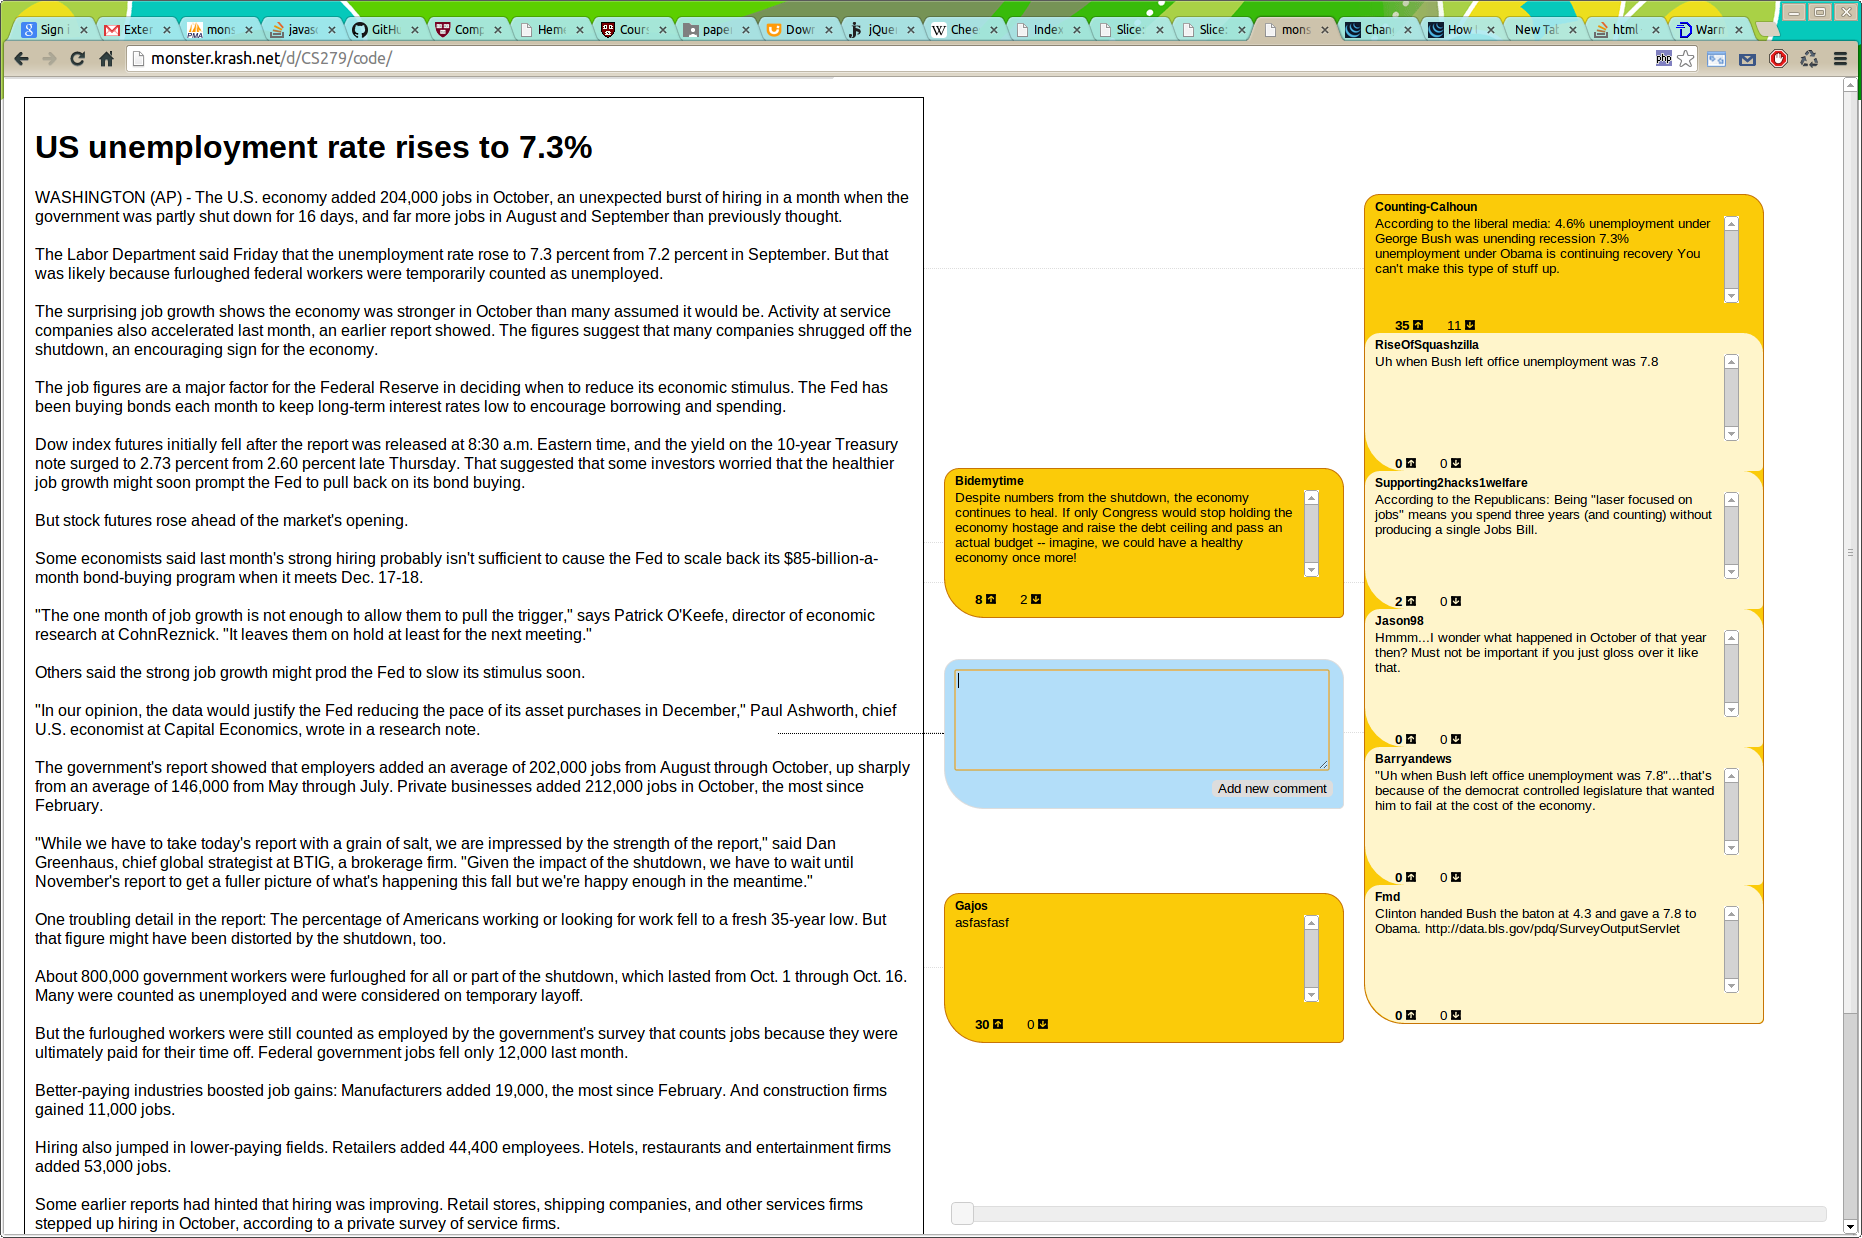
\includegraphics[scale=0.3]{mindmargin.png} 
\caption{The MindMargin system consists of a web client (shown here) and a server side back-end.}
\label{fig:frontend}
\end{figure}

Figure \ref{fig:traditional} shows the traditional vertical commenting system. The reference media is on top and the commenting system is placed below. Navigation within the article as well as within the comments can be performed via top/down scrolling. The organization of replies and up- and down-voting is similar to the MindMargin prototype.

\begin{figure}
\centering
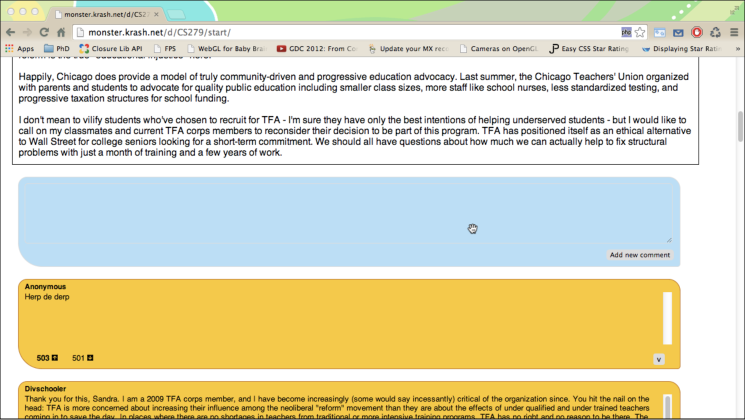
\includegraphics[scale=0.3]{traditional.png} 
\caption{The traditional comment system with a vertically ordered design.}
\label{fig:traditional}
\end{figure}

The front-ends were written in JavaScript using the popular jQuery and jQuery UI libraries. A model-view-controller pattern was chosen to structure the application code base. The user interface itself were created to adjust responsively to any window size.

\subsection{Back-end}
The server component of MindMargin and the traditonal system was written in PHP and communicates with the front-end and a relational database. Communication with the front-end is ensured by providing a REST-API which can be called via AJAX. The entity model of the client is replicated on the server. Data is read and stored using a custom and fully generalized object-relational-mapper. We chose MySQL for our database with a table each for users and comments.

Throughout the implementation, we followed an iterative approach to programming our software. The developer team was small. All developed code is released under the BSD open source license on github.


\section{Plan}

\begin{itemize}
\item \textbf{Milestone 1 (10/31/2013)}
\begin{itemize}
\item Complete relevant literature review research
\item Explore other methods for measuring engagement (in addition to sharing articles)
\item Design experiment and identify method of targeting participants (Question to be answered: how will we get people to participate?)
\item Compile a summary of existing commenting platforms and their features (http://www.hongkiat.com/blog/3rdparty-comment-discuss-systems-reviewed/)
\end{itemize}

\item \textbf{Milestone 2 (11/05/2013)}
\begin{itemize}
\item Prepare working prototype 
\item Two different commenting systems -- identify which features are constant
\begin{itemize}
\item Vertical (existing)
\item Horizontal (novel)
\end{itemize}
\item Complete relevant literature review research
\item Explore other methods for measuring engagement (in addition to sharing articles)
\item Design experiment and identify method of targeting participants (Question to be answered: how will we get people to participate?)
\item Compile a summary of existing commenting platforms and their features (http://www.hongkiat.com/blog/3rdparty-comment-discuss-systems-reviewed/)
\end{itemize}

\item \textbf{Milestone 3 (11/12/2013}
\begin{itemize}
\item Describe, design and execute experiment 
\item Begin data collection
\end{itemize}

\item \textbf{Milestone 4 (11/19/2013}
\begin{itemize}
\item Organize preliminary results
\item Analyze data and compare with hypotheses
\item Draw conclusions
\end{itemize}

\item \textbf{Milestone 5 (11/26/2013}
\begin{itemize}
\item Revise all sections for final review
\end{itemize}

\end{itemize}


\bibliographystyle{acm-sigchi}
\bibliography{lit}
\end{document}
